\documentclass{standalone}
\usepackage{tikz}

\begin{document}
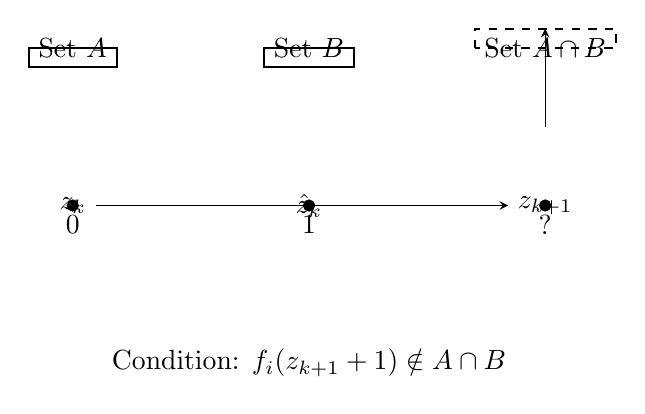
\begin{tikzpicture}[node distance=2cm, auto]

    % Define nodes
    \node (A) at (0,0) {Set \( A \)};
    \node (B) at (3,0) {Set \( B \)};
    \node (C) at (6,0) {Set \( A \cap B \)};
    
    % Draw sets
    \draw[thick] (A.west) rectangle (A.east |- C.south);
    \draw[thick] (B.west) rectangle (B.east |- C.south);
    \draw[dashed, thick] (C.west) rectangle (C.east |- A.north);
    
    % Define points
    \node (zk) at (0,-2) {$z_k$};
    \node (zkh) at (3,-2) {$\hat{z}_k$};
    \node (zkplusone) at (6,-2) {$z_{k+1}$};
    
    % Draw points
    \filldraw (zk) circle (2pt) node[below]{$0$};
    \filldraw (zkh) circle (2pt) node[below]{$1$};
    \filldraw (zkplusone) circle (2pt) node[below]{?};
    
    % Draw arrows
    \draw[-stealth] (zk) -- (zkplusone);
    \draw[-stealth] (zkplusone) ++(0,1) -- (zkplusone|-C.north);
    
    % Add labels
    \node at (3,-4) {Condition: \( f_i(z_{k+1} + 1) \notin A \cap B \)};
    
\end{tikzpicture}
\end{document}